%%%%%%%%%%%%%%%%%%%%%%%%%%%%%%%%%%%%%%%%%%%%%%%%%%%%%%%%%%%%%%%%%%%%%%%%%%%%%%
%
% タイトル TeX用テンプレート 
% バージョン 2014-11-8 (Sat) 初版
% 作成者 Kouhei Ito
% 作成場所 野々市市中林 DeuxMKK
% 用途 2段組レポートの作成等
%
%%%%%%%%%%%%%%%%%%%%%%%%%%%%%%%%%%%%%%%%%%%%%%%%%%%%%%%%%%%%%%%%%%%%%%%%%%%%%%%%
%\documentclass[11pt,twocolumn]{jsarticle}
%\documentclass[11pt]{jreport}
%\usepackage[dvipdfmx]{graphicx}
%\usepackage{amsmath,amssymb}
%\usepackage{url}
%\usepackage{nidanfloat}

\documentclass[twocolumn,11pt]{sotsuken_abst}

%% 体裁

% ページレイアウト(A4:297 mm × 210 mm,1 インチ = 25.4 mm)
% http://www.biwako.shiga-u.ac.jp/sensei/kumazawa/tex/layout.html
% http://www.slis.tsukuba.ac.jp/~fujisawa.makoto.fu/cgi-bin/wiki/index.php?TeX%A5%E1%A5%E2#p61e1b46
% 上 20 mm,下 22 mm,左右 20 mm の余白設定
\setlength{\topmargin}{-20truemm}
\setlength{\headheight}{10truemm}
\setlength{\headsep}{4.6truemm}
\setlength{\textheight}{255truemm}
\setlength{\oddsidemargin}{-5.4truemm}
\setlength{\evensidemargin}{-5.4truemm}  % twoside オプション指定時のみ有効
\setlength{\textwidth}{170truemm}
% \setlength{\columnsep}{8truemm}
\setlength{\columnsep}{6truemm}


%%%%%%%%%%%%%%%%%%%%%%%%%%%%%%%%%%%%%%%%%%%%%%%%%%%%%%%%%%%%%%%%%%%%%%%%%%%%%%%%
\title{超低重心6輪独立懸架ローバーの画像情報による自律走行}
\author{金沢工業高等専門学校 佐々井翔也,戸澗健,畠中和久}
\date{2016-12-20}
%%%%%%%%%%%%%%%%%%%%%%%%%%%%%%%%%%%%%%%%%%%%%%%%%%%%%%%%%%%%%%%%%%%%%%%%%%%%%%%%
\setcounter{page}{13}
\lhead{}
\chead{}
\rhead{{\sf 12・207}\\{\bf 機械工学科}}
\lfoot{}
\cfoot{{\sf-\ M-\thepage \ -}}
%\rfoot{}
\renewcommand{\headrulewidth}{3pt}
%\renewcommand{\footrulewidth}{1pt}

\begin{document}
%\layout
\maketitle
\thispagestyle{fancy}
\pagestyle{fancy}

\setlength{\baselineskip}{5.6truemm}
\kanjiskip=.07zw plus 3pt minus 3pt
\xkanjiskip=.07zw plus 3pt minus 3pt

%%%%%%%%%%%%%%%%%%%%%%%%%%%%%%%%%%%%%%%%%%%%%%%%%%%%%%%%%%%%%%%%%%%%%%%%%%%%%%%%
\section{緒言}
\subsection{研究の背景}
%そこで今回は走破性の向上を考え,前年度の改善案として低重心化とそれを補佐する懸架装置に注目し,”超低重心6輪独立懸架ローバー”を制作する
前年度つくばチャレンジ2015で使用したロボットの重心が高かったため,凸凹道やコンクリートなどでロボットが傾きそのまま転倒しかける様子が見られた.
そこで今回は走破性の向上を考え,前年度の改善案を元にロボットを開発する.また,ロボットが市街で自律走行を行うためには,自身の位置を推定する手段が必要である.その手段としてローカルマップをグローバルマップに変換する方法が一般的だ.
これらを行うために測域センサーを用いるのが主流である.しかし,今年度はローカルマップの生成を単眼カメラによって行おうと考えた.その理由としては,カメラは低コスト,省スペース,軽量であることが挙げられる.またローカルマップを生成するためには周囲との位置関係を求める必要がある.
カメラでは対象物を写した2枚の画像とそれらの画像間距離から三角測量の原理を用いることで対象物からカメラまでの距離を計測することができる.今回は単眼カメラを用いるため画像間距離はカメラの移動量に等しい.よってカメラの移動量を取得することができれば対象物との位置関係が分かる.

\subsection{研究の目的}
今年度は走破性の向上を考え,前年度の改善案として低重心化とそれを補佐する懸架装置に注目し,”超低重心6輪独立懸架ローバー”を開発する.またカメラの移動量をモーションセンサから得られる位置情報によって取得し,三角測量を行う.これを複数回行い,得られたデータをマップとする.


\section{ハードウェアの概要}
\subsection{走行モジュール}
設計した走行モジュールのCADを図\ref{fig:cad}に示す。図から確認できるように全高がタイヤ直径である190mm内に収まっているため低重心化が達成された.また6輪に付属している懸架装置を図\ref{fig:kenka}に示す.ばねを2本設置することでサスペンションとし,またそれらの取り付け位置を斜めにすることでさらに低重心が可能となった.

\begin{figure}[htp]
 \begin{center}
  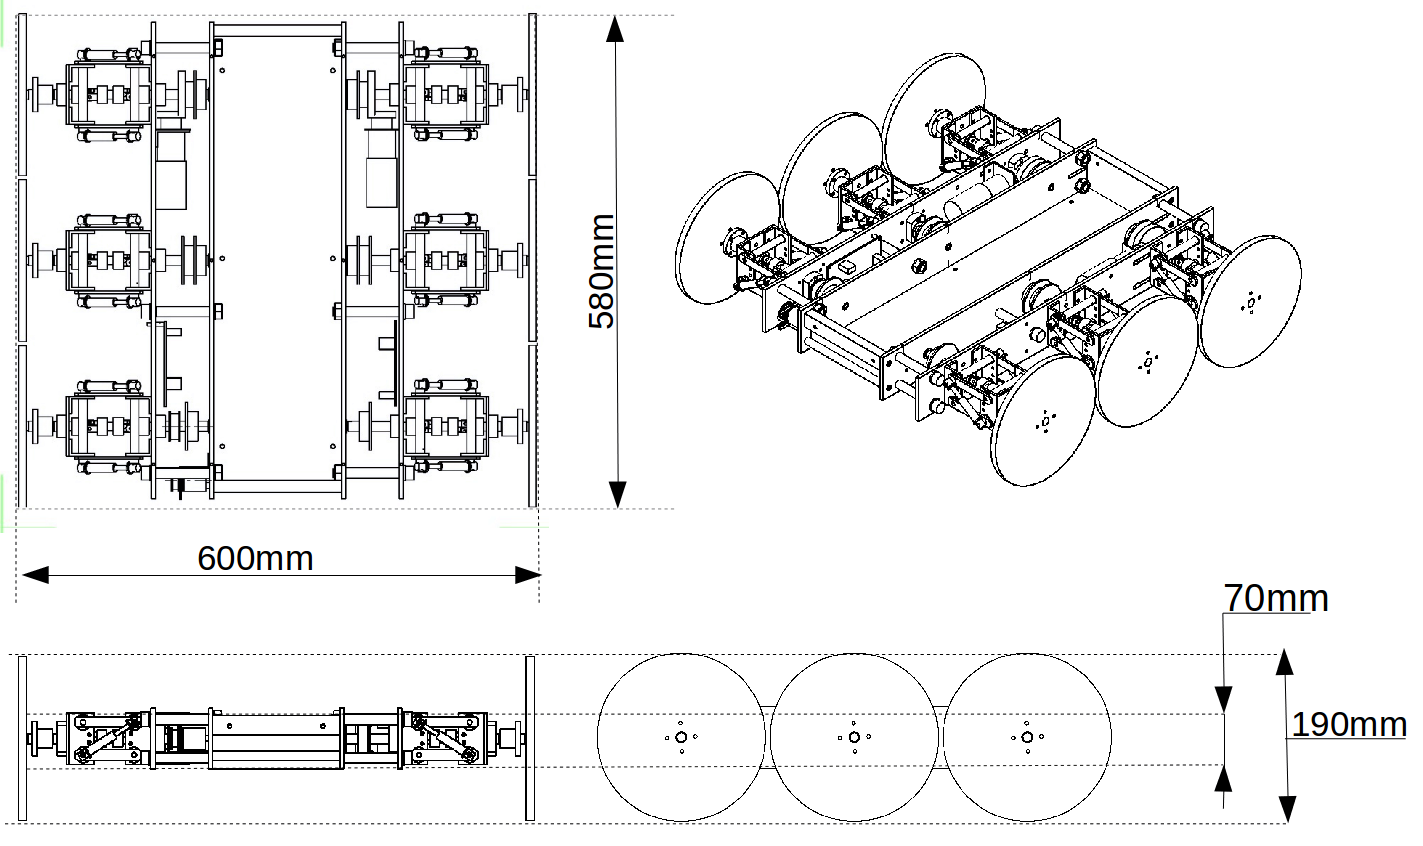
\includegraphics[width=70mm]{4.png}
  \caption{走行モジュール}
  \label{fig:cad}%ここに文章中で使用する名前を指定する
 \end{center}
\end{figure}

\begin{figure}[htp]
 \begin{center}
  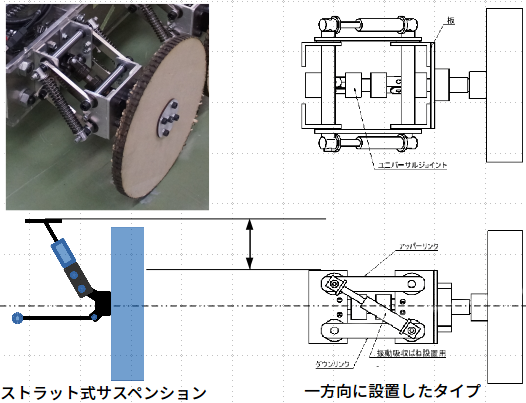
\includegraphics[width=70mm]{3.png}
  \caption{懸架装置}
  \label{fig:kenka}%ここに文章中で使用する名前を指定する
 \end{center}
\end{figure}

\subsection{ロボットの構成}
今年度のロボットに搭載したセンサを以下の表\ref{tab:op}に示す.



\subsection{超堤・超壕実験}
今回作成したロボットの性能を調査するため,超堤・超壕実験を行った結果,超堤:110[mm],超壕220[mm]が得られた.

\begin{table}[h]
  \begin{center}
    \caption{ハードウェアの構成}
    \small
  \scalebox{0.85}{
  \begin{tabular}{|c|c|} \hline
    構成要素 & メーカ・型番・スペックなど \\ \hline
    Mian PC & NVIDIA JETSON TK1 \\ \hline
    OS & Ubuntu 14.04 LTS \\ \hline
    camera & Panasonic HX-A1H \\ \hline
    Buttery & KyPOM KT5100 4S 35C \\ \hline
    Motor & MABUCHI MOTOR RS-555VC-5524 \\ \hline
    Motion Sensor & 東京航空計器株式会社 CSM-MG100\\ \hline

  \end{tabular}
  }
    \label{tab:op}
  \end{center}
\end{table}

\section{マップ生成}
\subsection{移動量の取得}
カメラの移動量を取得するため,東京航空計器社製のモーションセンサから得られる位置情報を使用する.モーションセンサーを図\ref{fig:motion}に示す.1回目に取得した位置と2回目に取得した位置の
差から移動量を算出する.

\begin{figure}[htp]
 \begin{center}
  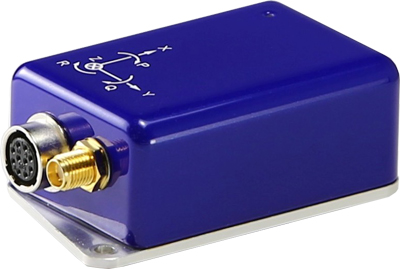
\includegraphics[width=30mm]{motion.jpg}
  \caption{モーションセンサー}
  \label{fig:motion}%ここに文章中で使用する名前を指定する
 \end{center}
\end{figure}

\subsection{マップ生成環境}
マップの生成環境を図\ref{fig:map}に示す.天候はカメラ画像に影響の少ないくもりの日,画像間距離を1.4[m]として金沢工業高等専門学校の駐車場付近でマップ生成を行った.ロボットはStart地点から矢印の方向に進み,2回の旋回を経てGoal地点まで走行する.

\begin{figure}[htp]
 \begin{center}
  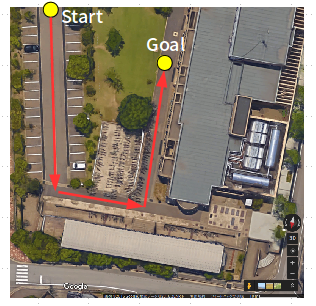
\includegraphics[width=50mm]{1.png}
  \caption{マップ生成環境}
  \label{fig:map}%ここに文章中で使用する名前を指定する
 \end{center}
\end{figure}

\subsection{マップ生成}
生成されたマップを図\ref{fig:mapp}に示す.赤い点群はカメラ画像から三角測量によって得られた周囲の位置関係,青い線はカメラ画像から得られたロボットの走行軌跡,黄色い線を実際にロボットが走行した軌跡である.
図より,カメラ画像からマップを生成することができた.
しかしカメラ画像から得られたロボットの走行軌跡は1回目の旋回時から,実際にロボットが走行した軌跡と比べて大きく歪んでいることが確認できる.

\begin{figure}[htp]
 \begin{center}
  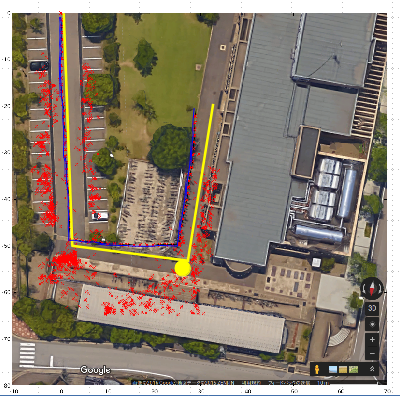
\includegraphics[width=50mm]{2.png}
  \caption{生成したマップ}
  \label{fig:mapp}%ここに文章中で使用する名前を指定する
 \end{center}
\end{figure}

\section{結言}
走破性の高いロボットの開発の実現にあたり,つくば市内での走行が問題なく行えたため,走破性の高いロボットの開発は達成したと考える.また移動量の取得とマップ生成の実現にあたり,生成したマップは旋回時に大きく歪むことが確認されたが直線時には問題がなかったため3次元復元技術の基礎は確立できたと考える.

% 参考文献
\begin{thebibliography}{8}
%  \bibitem{harris} LandingProducts, APCPro\nolinebreak pellers,\nolinebreak
%http://www.\linebreak apcprop. com{\slash}v{\slash}index.html,
%2012/8/21
%\bibitem{kyonenn} GPS測位計算プログラム入門,ROS,http://www.enri.go.jp/~fks442/K_MUSEN
\bibitem{ros} Bradski,Kaehler:詳解 OpenCV,433,株式会社オライリー・ジャパン(2012)
\bibitem{kyonenn} 理解するためのGPS測位計算プログラム入門,http://www.enri.go.jp/~fks442%/K_MUSEN
%  \bibitem{koukuu} 中村 資郎:新航空工学講座 第7巻 プロペラ:日本航空技術協会,pp.23-24,1988
%  \bibitem{rikigaku} 加藤 寛一郎,大屋 昭男,柄沢 研治:航空機力学入門,東京大学出版会,pp.32,1982
\end{thebibliography}

%%%%%%%%%%%%%%%%%%%%%%%%%%%%%%%%%%%%%%%%%%%%%%%%%%%%%%%%%%%%%%%%%%%%%%%%%%%%%%%%


\end{document}
